\documentclass[french]{article}


\usepackage[utf8]{inputenc} % encode en UTF8

\usepackage[T1]{fontenc}





\usepackage[top=2cm, bottom=2cm, left=3cm, right=3cm]{geometry}
\usepackage{graphicx}
\usepackage{caption}
\usepackage{subcaption}
\usepackage{float}
\graphicspath{ {./photo/} }

%Belles fraction de fration \cfrac
\usepackage{amsmath}

\usepackage{tikz}
\usepackage{circuitikz}




\newcommand{\HRule}{\rule{\linewidth}{0.5mm}} % Epaisseur des lignes horizontales

\pagestyle{empty}
\newcommand{\myTitle[1]}{
\begin{minipage}{.47\textwidth}
\centering
\begin{flushleft}

\includegraphics[width=0.75\textwidth]{./photo/nantes_universite_logo.png}
\end{flushleft}
\end{minipage}
\begin{minipage}{.47\textwidth}
\centering
\begin{flushright}
\hspace*{1cm} 
\includegraphics[width=0.85\textwidth]{./photo/logo_polytech_nantes}
\end{flushright}
\end{minipage}~\\[1.5cm]

\begin{center}
\vspace*{\stretch{0.3}}
\end{center}

\begin{center}
  \Large
  \vspace*{\stretch{1}}
  \HRule \\[0.2cm]
  \begin{center}
    \huge
    \textbf{#1}\\ %Titre
  \end{center}
  %\textbf{\\ Projet Transversal}\\ %matière
  \HRule \\[1.5cm]
  
%  \vspace*{\stretch{5}}
%  
%  \small
%  \noindent Rédigé par \\
%  \vspace*{\stretch{0.2}}
%  \large
%  \noindent \Redac\\
%  \vspace*{\stretch{0.5}}
 
\end{center}

\vspace*{\stretch{2}}

\begin{center}\large
	\textsc{École Polytech de Nantes}\\
	\textsc{Département Électronique et Technologie du Numérique}
\end{center}

\vspace*{\stretch{5}}

\begin{center}
	\begin{minipage}{0.4\textwidth}
		\begin{flushleft} \large
        	\noindent Rédigé par\\ %\Redac
			Victor DUFRENE \\
			Mathis BRIARD\\
			Louison GOUY\\
			Yujie HUANG
		\end{flushleft}
	\end{minipage}
	\begin{minipage}{0.4\textwidth}
		\begin{flushright}\large
			Professeur encadrant : \\Yann MAHE\\ Anne CHOUSSEAUD\\
						
		\end{flushright}
	\end{minipage}
\end{center}
}

\begin{document}
\myTitle[Rapport de mini-projet \\ - Électronique Hautes Fréquences - ]
\newpage

\section{Résumé}


\newpage

\section{Synthèse de filtre passe-bas en technologie }


L'objectif est de réaliser un filtre passe-bas dont le gabarit est donné à la figure \ref{fig:gabarit_PasseBas} avec une réponse de Tchebychev.

\begin{figure}[H]
	\centering
	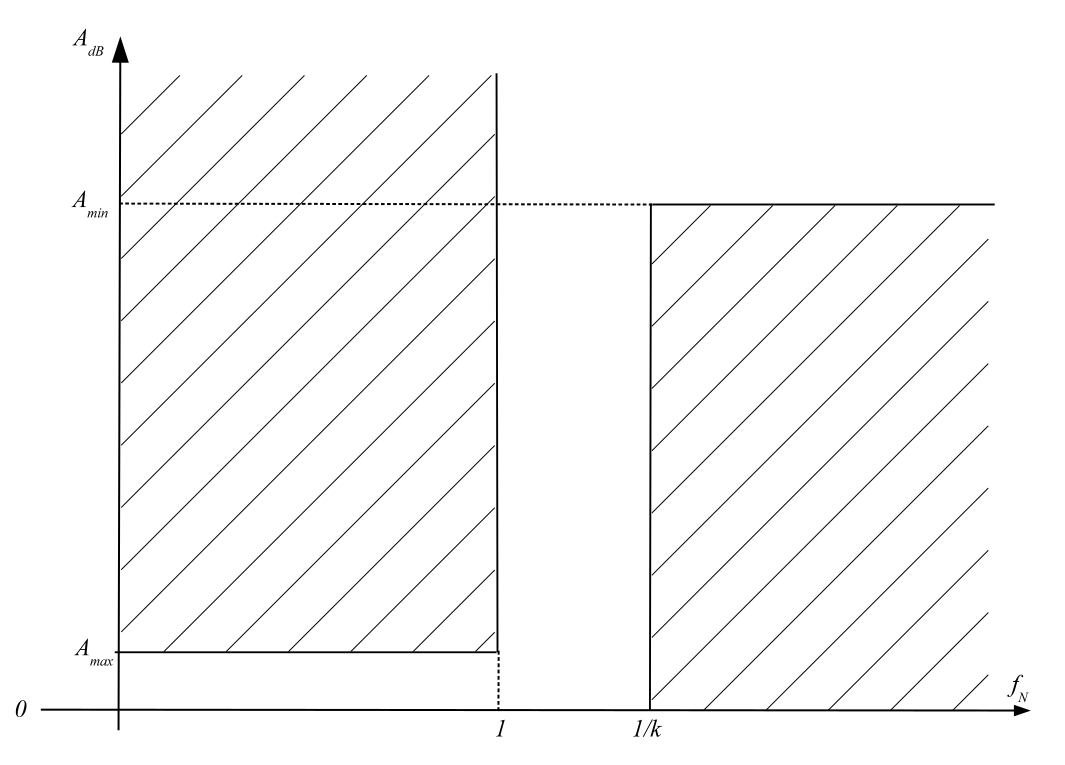
\includegraphics[width=0.5\linewidth]{ressources/gabarit_passe_pas}
	\caption{Gabarit filtre passe bas équivalent}
	\label{fig:gabarit_PasseBas}
\end{figure}

Les valeurs numériques associées au gabarit sont les suivantes.
\begin{table}[H]
	\centering
	\begin{tabular}{|p{1.5cm}|p{1.5cm}|p{1.5cm}|p{1.5cm}|}
		\hline
		$A_{max}$& $A_{min}$ & $f_s$ & $f_c$ \\ \hline
		0.1	dB & 15,00 dB 		& 2 GHz	   & 3 GHz \\ \hline
	\end{tabular}
	\caption{Valeur numérique gabarit souhaité}
\end{table}


La conception d'un filtre hautes fréquences débute par une synthèse classique avec des éléments passifs (condensateurs et bobines) comme il a été fait dans le module moyennes fréquences du S7. A partir du gabarit de la figure \ref{fig:gabarit_PasseBas}, l'équation ci-dessous nous est permet d'obtenir l'ordre du filtre à concevoir.



\begin{equation}
	n \geq \cfrac{argch(\sqrt{\cfrac{\alpha_{min}-1}{\alpha_{max} -1}})}{argch(1/k)}
\end{equation}
On rappelle :
\begin{equation}
argch(x)=ln(x+\sqrt{x^2-1})
\end{equation}

Où :
\begin{itemize}
	\item n est l'ordre du filtre souhaité;
	\item k est la sélectivité égal à : 
	\begin{equation}
		k=\frac{f_s}{1,5f_s} = \frac{2}{3} \approx 0,67
	\end{equation}
	\item $\alpha_{min}$ est l'atténuation minimale (en linéaire) du signal dans la bande atténué égal à $10^{\frac{15}{10}} \approx 31,6$
	\item $\alpha_{max}$ est l'atténuation maximale (en linéaire) du signal dans la bande passante égal à $10^{\frac{0,1}{10}} \approx 1,02$
\end{itemize}

L'application nous donne $n \geq 4,5$ soit au minimum un ordre 5 pour respecter le gabarit souhaité. Le schéma passe-bas en impédance que nous allons utiliser est donné ci-dessous par la figure \ref{fig:gabarit_PB}.

\begin{figure}[H]
	\centering
	\begin{circuitikz}
		\draw (0,0)
		to[V,v=$U_e$] (0,2) % The voltage source
		to[L=$g_1$] (2,2)
		to[C=$g_2$] (2,0) % The resistor
		(2,2)to[L=$g_3$] (4,2)
		to[C=$g_2$] (4,0) % The resistor
		(4,2)to[L=$g_3$] (6,2)
		to [R=$r$] (6,0) 
		to[short] (0,0);
	\end{circuitikz}
	\caption{Schéma prototype d'un filtre passe-bas de Tchebycheff en impédance.}
\end{figure}

Avec :
\begin{itemize}
	
	\item les coefficients $g_k$, les valeurs normalisées des condensateurs et des bobines;
	\item r, la résistance de charge normalisée est égale à 1. Sa valeur dénormalisé est de $50\Omega$;
	\item $U_e$, le signal d'entrée ayant une résistance série normalisée égale à 1 et donc $50\Omega$ en dénormalisée.
\end{itemize}

Pour obtenir les valeurs de $g_k$ nous ne pouvons utilisé les tableaux données dans le polycopié d'électronique moyennes fréquences car ils ne sont valables uniquement pour des ondulations de 0.5 dB et 1 dB. Notre gabarit nous impose une ondulation maximale de 0.1 dB dans la bande passante. Pour obtenir des coefficient $g_k$ qui permettent de respecter l'ondulation voulue nous avons réalisé un script sur Octave disponible en annexe. Le résultat obtenu est le suivant.

\begin{table}[H]
	\centering
	\begin{tabular}{|p{2cm}|p{2cm}|p{2cm}|p{2cm}|p{2cm}|}
		\hline
		$g_1$ & $g_2$ & $g_3$ & $g_4$ & $g_5$\\
		\hline
		1.1468 & 1.3712 & 1.9750 & 1.3712 & 1.1468\\
		\hline
	\end{tabular}
	\caption{Valeurs des composants normalisées pour une ondulation de 0.1 dB}
	\label{tab:coefficient_g_k_passe_bas}
\end{table}
 
Pour trouver les valeurs réelles des composants il faut : pour les condensateurs, multiplier les $g_k$ pairs par un coefficient $C_{denom}$ et pour les bobines, multiplier les $g_k$ impairs par un coefficient $L_{denom}$. Les valeurs de ces coefficients sont données ci-dessous.

\begin{equation}
	C_{denom} = \frac{1}{2\pi f_s R}
	\qquad
	L_{denom} = \frac{R}{2\pi f_s}
\end{equation}

Le tableau ci-dessous donne les applications numériques pour les composants du filtre avec $f_c = 2GHz$ et $R = 50\Omega$.

\begin{table}[H]
	\centering
	\begin{tabular}{|p{2cm}|p{2cm}|p{2cm}|p{2cm}|p{2cm}|}
		\hline
		$L_1$ & $C_2$ & $L_3$ & $C_4$ & $L_5$\\
		\hline
		4.56 nH & 2.18 pF & 7.86 nH & 2.18 pF & 4.56 nH\\
		\hline
	\end{tabular}
	\caption{Valeurs réelles des composants du filtre passe-bas.}
	\label{tab:valeurs_composant_passe_bas}
\end{table}




\section{synthèse d'un filtre passe-bande}

La synthèse d'un filtre en hautes fréquences à partir d'un gabarit se rapporte à la méthode étudiée en moyenne fréquence. Une étape finale est ajoutée permettant la transformation des éléments localisés en éléments distribués.
Le cahier des charges est le suivant, concevoir un filtre passe bande basé sur une fonction d'approximation de type Tchebychev et respectant le gabarit figure \ref{fig:gab}. L'implémentation réelle doit se en utilisant exclusivement des lignes micro ruban de longueur $\lambda_g/2$ ou $\lambda_g/4$ et des stubs.

\begin{figure}[H]
	\centering
	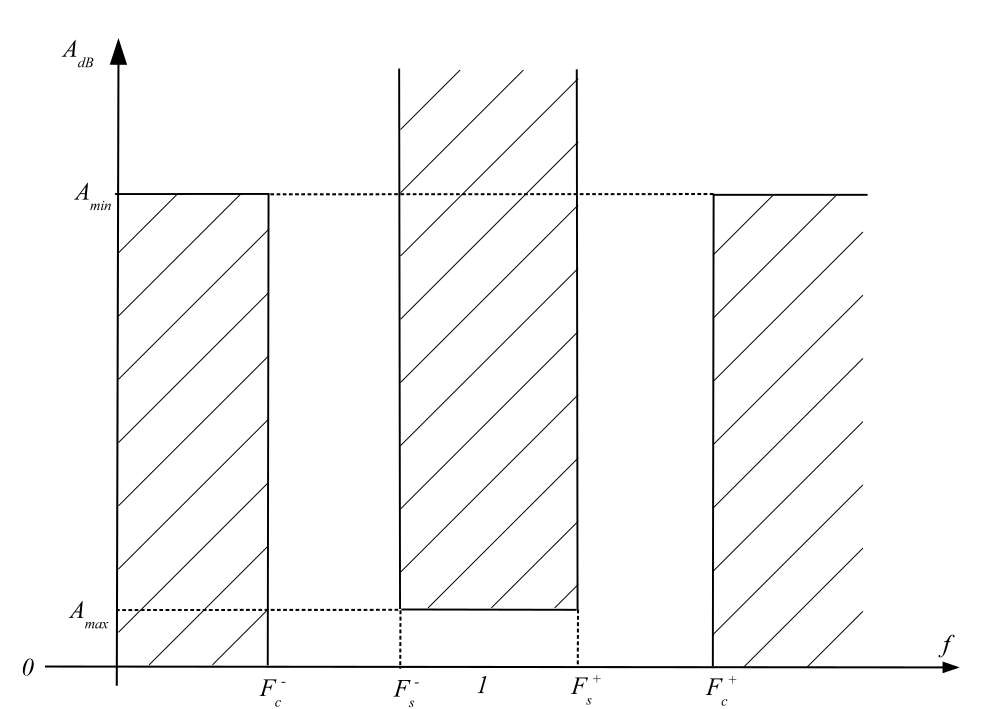
\includegraphics[width=0.5\linewidth]{ressources/gabarit_passe_bande}
	\caption{Gabarit du filtre passe-bas souhaité}
	\label{fig:gab}
\end{figure}
Les valeurs numériques associées au gabarit sont les suivantes. Les fréquences sont en GHz et l'atténuation en dB. 
	\begin{table}[H]
		\centering
\begin{tabular}{|c|c|c|c|c|c|}
		\hline
	$A_{max}$& $A_{min}$ & $f_c^-$ & $f_s^-$ & $f_s^+$ &$f_c^+$ \\ \hline
	0,1000	 & 15,00 		& 1,500	   & 1,750 & 2,250& 3,000 \\ \hline
	\end{tabular}
\caption{Valeur numérique gabarit souhaité}
	\end{table}
\paragraph{Symétrie du gabarit} ~~\\ \noindent
Avant de commencer la synthèse du filtre il est nécessaire de valider une condition sur la symétrie. Si elle n'est pas respectée il faudra modifier le gabarit du cahier des charges. La condition s'opère sur la moyenne géométrique de la bande passante et de la bande coupée notées :
\begin{equation}
	 f_{co} = \sqrt{f_c^-.f_c^+}, \quad f_{so} = \sqrt{f_s^- f_s^+}
\end{equation}
Ainsi, si $f_{so} = f_{co}$, le gabarit est centré il n'est pas nécessaire de réaliser d'opération particulaire. On obtient a alors  $f_{so} = f_{co} = f_0$ avec $f_0$ la fréquence centrale du gabarit. Si $f_{so} \neq f_{co}$, le gabarit n'est pas centré il faut passer par une étape de centrage du gabarit avant de réaliser la synthèse du filtre.\\
Application numérique :\\
\begin{equation}
f_{co} = \sqrt{f_c^-.f_c^+} = \sqrt{1,500*3,000} = 2,121 GHz
\end{equation}
\begin{equation}
	f_{so} = \sqrt{f_s^- f_s^+} = \sqrt{1,750*2,250} = 1,984 GHz
\end{equation}
\begin{equation}
f_{so} <	f_{co}
\end{equation}
Le filtre est asymétrique il faut réaliser l'opération de centrage. Dans notre cas elle vise à diminuer $f_{co}$. Il est possible de faire varier la borne positive $f_c^+$. Cela à pour effet de sur contraindre le cahier des charges. Pour répondre aux exigences il est interdit d'élargir la bande atténué ou de diminuer la bande passante. Ainsi on fixe la fréquence centrale $f_0 = f_{so} = \sqrt{f_s^- f_s^+}$.  
Il vient donc :
\begin{equation}
f_c^+=\frac{f_{so}^2}{f_c^-}=\frac{1,984^2}{1,500}=2,614GHz
\end{equation}
Les nouvelles valeurs numériques pour le gabarit du filtre sont les suivantes. Elle font référence à la figure \ref{fig:gab}.
	\begin{table}[H]
	\centering
	\begin{tabular}{|c|c|c|c|c|c|c|}
		\hline
		$A_{max}$& $A_{min}$ & $f_c^-$ & $f_s^-$ & $f_0$ & $f_s^+$ &$f_c^+$ \\ \hline
		0,1000		 & 15,00 		& 1,500	   & 1,750 & 1,984 & 2,250& 2,614 \\ \hline
	\end{tabular}
	\caption{Valeur numérique gabarit centré}
\end{table}
\paragraph{Gabarit passe bas} ~~\\ \noindent
L'étape suivant dans la conception d'un filtre passe bande symétrique vise à simplifier la synthèse en passant par un gabarit passe bas. Cela permet de calculer son ordre puis sa structure en éléments localisés.
\begin{figure}[H]
	\centering
	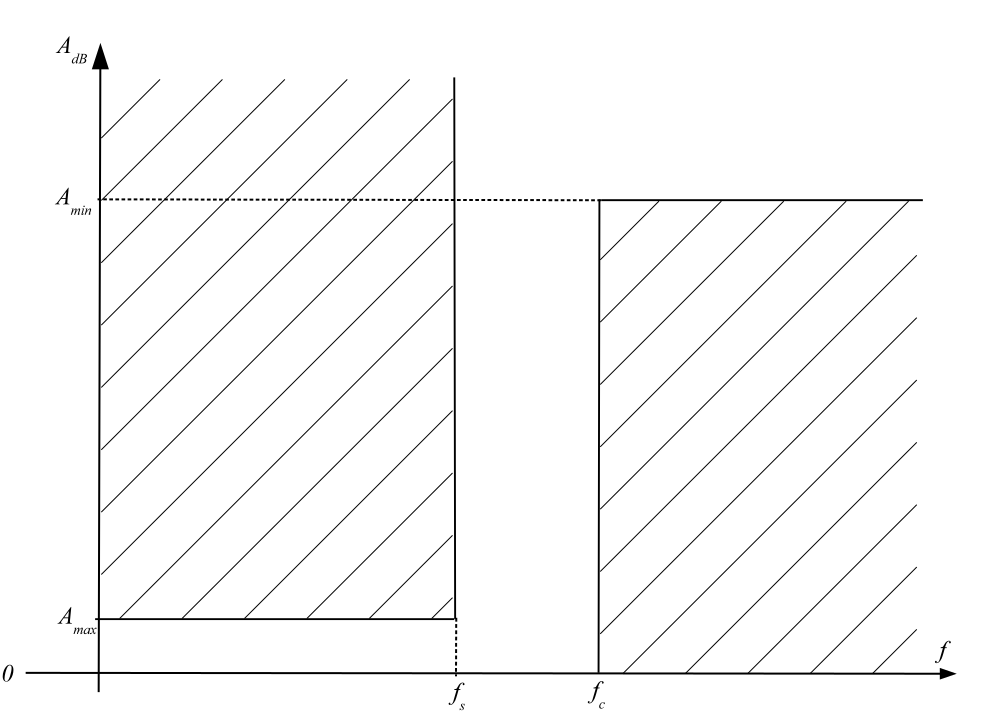
\includegraphics[width=0.5\linewidth]{ressources/gabarit_passe_bas}
	\caption{Gabarit filtre passe bas équivalent}
	\label{fig:gabaritpassepas}
\end{figure}
L'évaluation du coefficient de sélectivité permet d'établir le gabarit normalisée. Cette grandeur se note $k$ est sans unité et strictement inférieure à 1. Son expression est la suivante :
\begin{equation}
	k=\frac{\Delta.f_s}{\Delta.f_c}=\frac{f_s^+-f_s^-}{f_c^+-f_c^-}=\frac{2,250-1,75}{2,614-1,500}=0,4488
\end{equation}
L'ordre du filtre $\delta \in N$ est donnée pour une fonction d'approximation de Tchebychev avec l'expression suivante. Les atténuations $A_{min}$ et $A_{max}$ en dB correspondent respectivement aux fréquences $f_s$ et $f_c$.
\begin{equation}
\delta \geq \frac{argch
	\Big( \sqrt{\cfrac{10^{A_{min}/10}-1}{10^{A_{max}/10}-1}}
	\Big)
}{argch(1/k)}
\end{equation}
On rappelle pour la calculatrice :
\begin{equation}
argch(x)=ln(x+\sqrt{x^2-1})
\end{equation}
On calcule avec $A_{min} = 15dB$ et $A_{max} = 0,1dB$. L'ordre $\delta$ est arrondi à l'entier supérieur.
\begin{equation}
\frac{argch
	\Big( \sqrt{\cfrac{10^{15/10}-1}{10^{0,1/10}-1}}
	\Big)
}{argch(1/0,4488)} = 2,975, \quad \delta = 3
\end{equation}
Le gabarit impose un ordre minimum de 3, c'est la valeur que nous retiendront. On note tout de même que l'arrondi au supérieur présente un faible écart avec l'ordre choisi. Notre filtre devrait respecter les spécifications mais des approximations pourraient entraîner des débordements notamment aux fréquences particulières $f_c$ et $f_s$.
\paragraph{Prototype passe bas normalisé vers passe bande dénormalisé} ~~\\ \noindent
Cette étape vise à transformer le schéma passe bas en son équivalent passe bande. Il existe deux schémas possibles dit de type impédance et de type admittance où, respectivement, le premier élément est une inductance ou un condensateur. Le cahier des charges ne donne pas d'indications sur ce point. Nous choisirons le schéma qui a l'avantage de simplifier la transposition micro ruban.
\begin{figure}[H]
	\centering
	\begin{circuitikz}[scale=0.8]
		\draw 
		(0,0) to[esource] (0,2) % The voltage source
		to [R=$1$] (3,2) 
		to[L=$l'_1$] (5,2)
		to[L=$l'_3$] (8,2)
		to [R=$r$] (8,0) 
		to[short] (0,0)
		(5.3,2)to[C=$c'_2$] (5.3,0);
	\end{circuitikz}
	\caption{Schéma prototype filtre passe-bas ordre 3 en admittance}
	\label{fig:ordre3_LP_adm}
\end{figure}
La figure \ref{fig:ordre3_LP_adm} représente le prototype du filtre passe bas. Il est composé de trois composants réactifs et le premier est une self, nous sommes bien en présence d'un filtre d'ordre trois de type impédance. Les valeurs normalisées de ces composants s'expriment à partir de l'atténuation maximum $A_{max}$, de l'ordre du filtre et de la charge. Dans le cas des ordres paires les deux résistances n'ont pas la même valeur, il est donc préférable de choisir un ordre impaire sans quoi une problématique d'adaptation se posera. Les calculs pour obtenir les valeurs des composants sont détaillés dans \cite{cours_MF} à la page 93. Ils font intervenir des fonctions trigonométriques relativement complexes. La figures \ref{fig:coefnormaliseondulation01db} ci-dessous rassemble ces grandeurs et nous évite les calcul. Elle correspond  à une ondulation inférieur à 0,1dB en bande passante et un ordre compris entre 1 et 10. 
\begin{figure}[H]
	\centering
	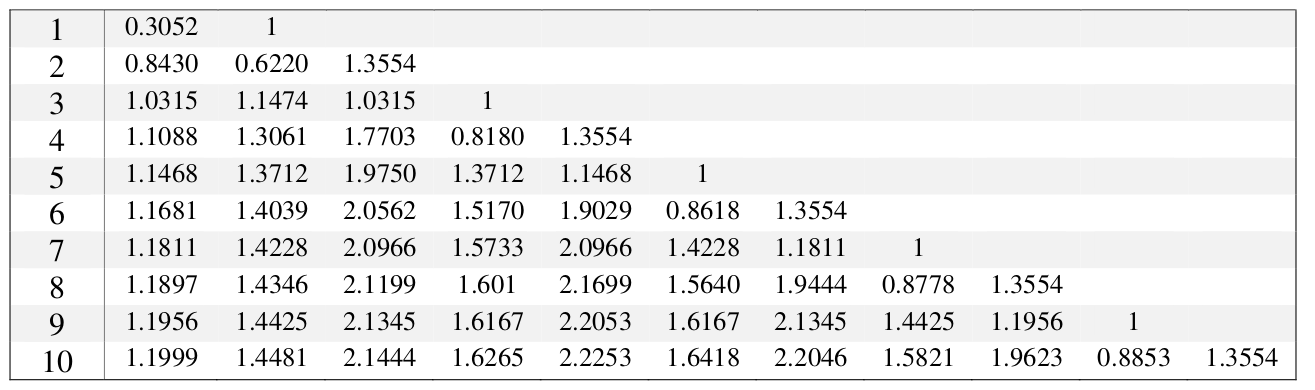
\includegraphics[width=0.8\linewidth]{ressources/coef_normalise_ondulation01dB}
	\caption{Coefficients normalisés fonction de Tchebychev 0,1dB ondulation}
	\label{fig:coefnormaliseondulation01db}
\end{figure}
La première colonne de ce tableau correspond à l'ordre du filtre. Les valeurs suivantes correspondent aux composants de gauche à droite sur le schéma. La dernière valeur concerne la résistance de charge. On remarque bien que pour les ordres impaire cette dernière vaut l'unité contrairement aux ordres impaires. Dans notre cas $l'_1=1,0315$, $c'_2=1,1474$ et $l'_3=1,0315$. Les informations nécessaires à la transformation du schéma équivalant passe bas au schéma équivalent passe bande ont été rassemblé. Nous pouvons opérer cette opération. Les éléments inductifs doivent être remplacés par une self et un condensateur en série. Les éléments capacitifs doivent être remplacés par une self et un condensateur en parallèle. Les valeurs normalisées des nouveaux composants sont données par les expressions suivantes:\\
Cas de l'inductance :
\begin{equation}
c_k=\frac{B}{l'_k}, \quad l_k=\frac{l'_k}{B}
\end{equation}
Cas du condensateur :
\begin{equation}
l_k=\frac{B}{c'_k}, \quad c_k=\frac{c'_k}{B}
\end{equation}
Où B désigne la bande passante
\begin{equation}
	B=\frac{\Delta f_s}{f_0}=\frac{f_s^+-f_s^-}{f_0}=\frac{2,250-1,75}{1,984}=0,2520
\end{equation}



\section{Conclusion}
Il existe une méthode détaillée dans le \textit{cours de filtrage actif} de Vincent Gouret faisant varier à la fois $f_{so}$ et $f_{co}$. Elle permet d'optimiser la contrainte sur le sélectivité. 












\end{document}
